\chapter{Phân tích Tương quan giữa FireAnt và Thị trường Chứng khoán Việt Nam}

\section{Khối lượng giao dịch cổ phiếu với Số lượng bài viết}

Đến với yếu tố đầu tiên mà chúng em muốn đề cập đến ở đây là liệu rằng có tồn tại mối tương quan nào giữa số lượng bài viết và khối lượng giao dịch của 3 chỉ số chứng khoán hàng đầu Việt Nam như VN30, VNINDEX, HNXINDEX. hay không.\\

Ta cùng nhìn qua 2 biểu đồ đã được đề cập từ trước, biểu đồ (\ref{fig:3.4}) thể hiện khối lượng giao dịch của VNINDEX, VN30, HNXINDEX và biểu đồ (\ref{fig:2.1}) thể hiện số lượng bài viết theo ngày:

\begin{figure}[H]
  \begin{subfigure}{.5\textwidth}
  \centering
    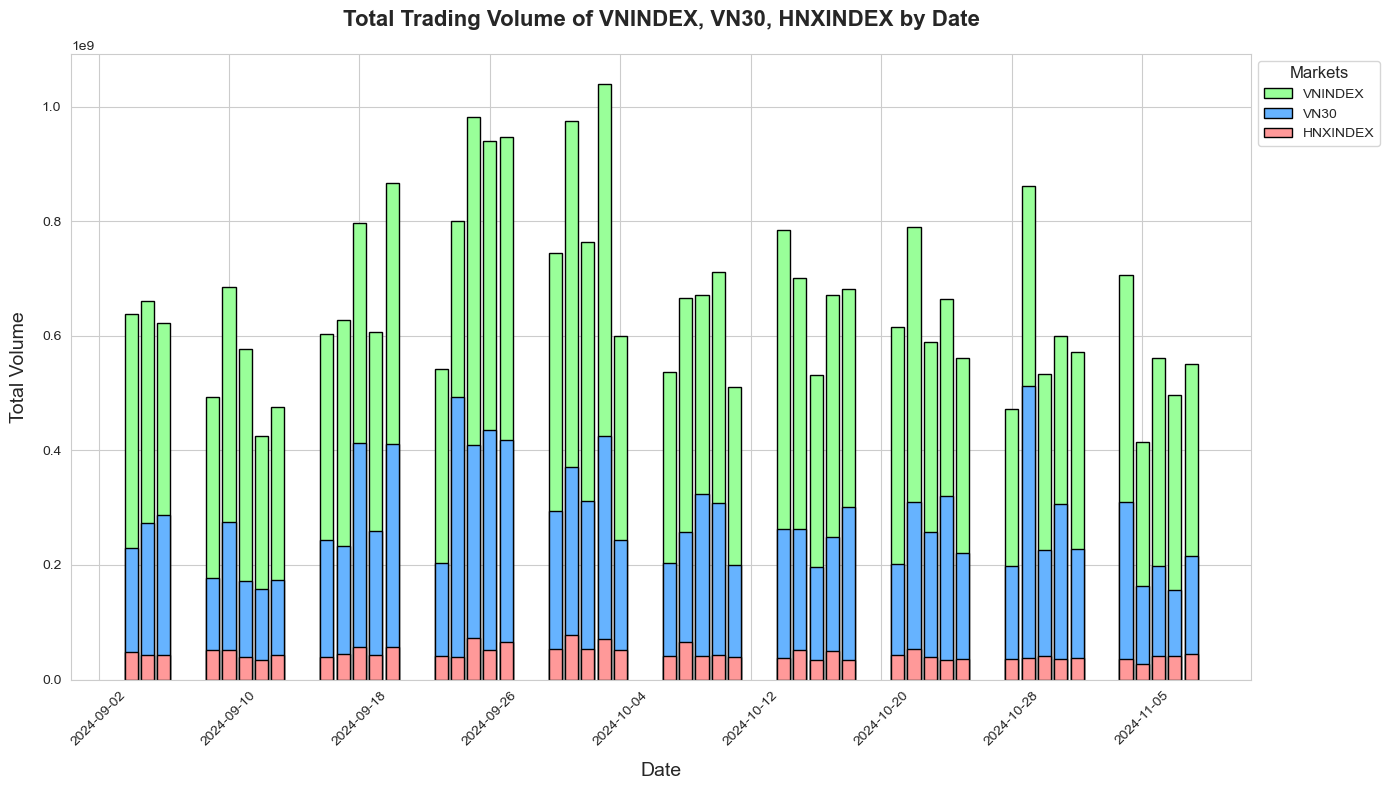
\includegraphics[width=1\linewidth]{images/plot-2.6-column_chart.png}
    \caption{Khối lượng giao dịch các chỉ số}
  \end{subfigure}%
  \begin{subfigure}{.5\textwidth}
  \centering
    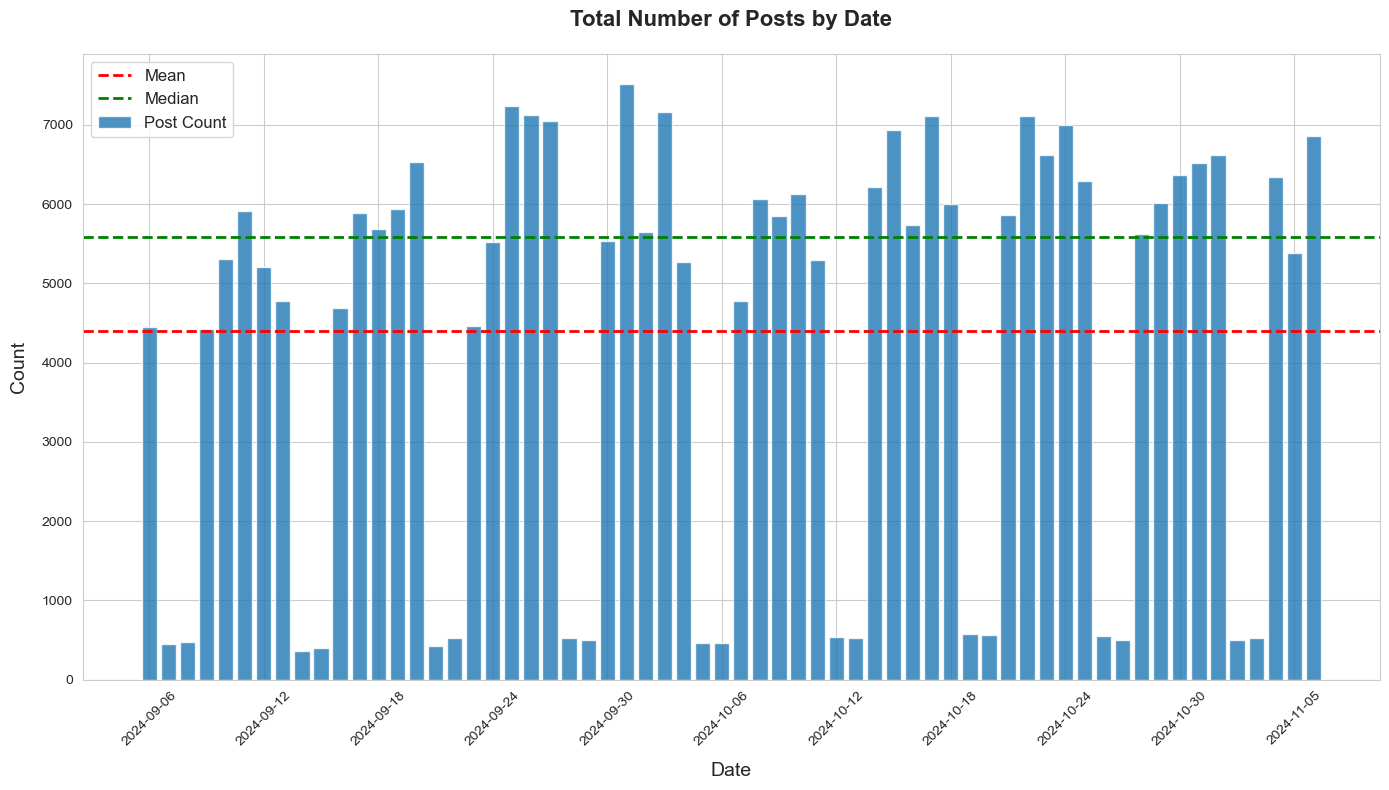
\includegraphics[width=1\linewidth]{images/plot-2.21-column_chart.png}
    \caption{Số lượng bài viết theo ngày}
  \end{subfigure}
\end{figure}

Dễ dàng nhận thấy có một sự tương đồng. Ta nhận xét và có thể đưa ra giả định rằng, khi số lượng bài viết tăng (đặc biệt nếu là ngày quan trọng), khối lượng giao dịch có thể tăng do nhà đầu tư chú ý và phản ứng với thông tin hay có xuất hiện sự kiện thu hút dòng vốn mới vào cổ phiếu liên quan. Ngược lại, nếu một cổ phiếu ít được chú ý (số lượng bài viết ít), khả năng khối lượng giao dịch sẽ thấp do sự quan tâm ít hơn.\\

Ta sẽ đặt giả thuyết rằng: Số lượng bài viết trong ngày có tương quan thuận với khối lượng giao dịch của thị trường.
Khi sử dụng Scatter plot, ta dễ thấy xu hướng đồng thuận hiện hữu, kết quả khá khả quan (hình \ref{fig:4.1}):\\

\begin{figure}[ht]
    \centering
        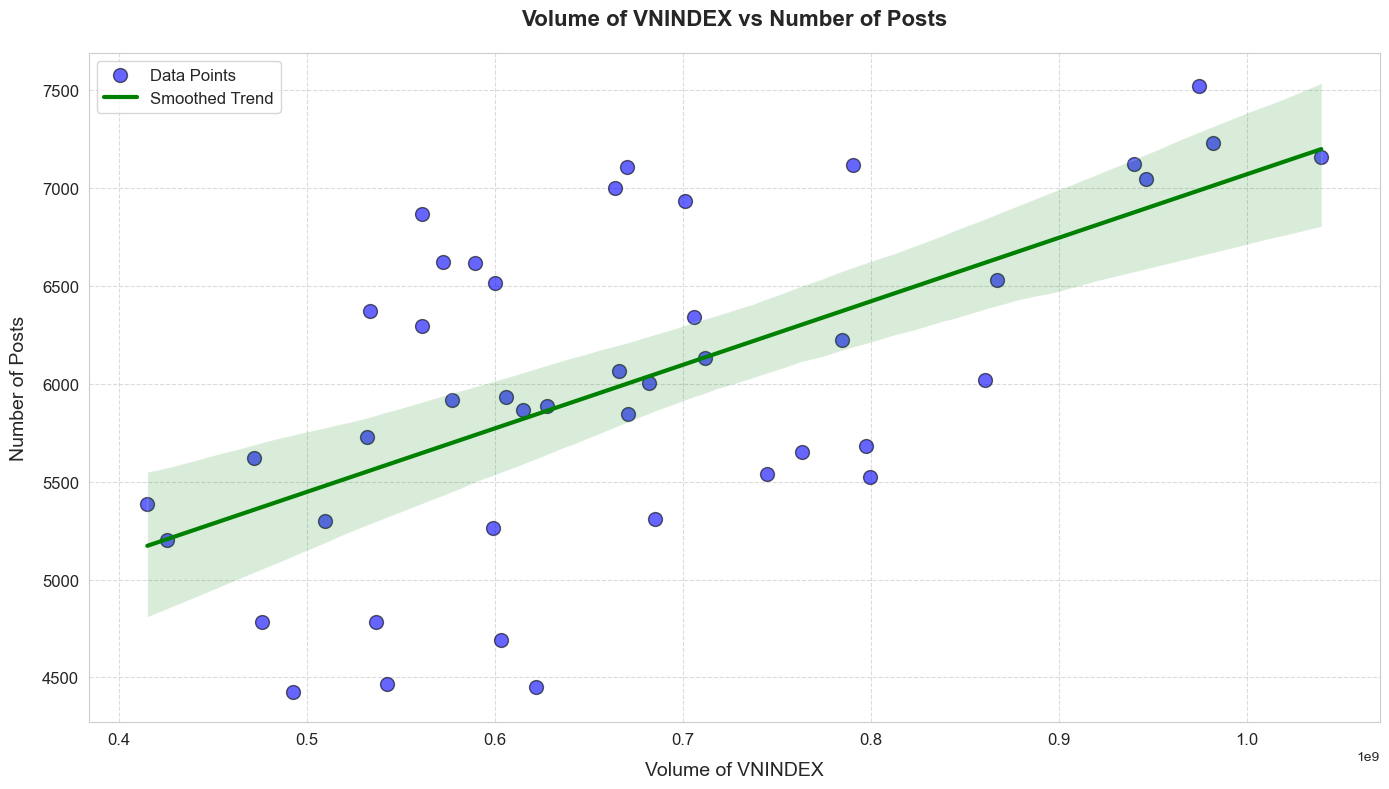
\includegraphics[width=0.75\linewidth]{images/plot-2.8-scatter_plot_smooth.png}
    \caption{Scatter plot với VNINDEX}
    \label{fig:4.1}
\end{figure}

Nhưng có vấn đề chỉ thực sự xuất hiện khi ta cố gắng chứng minh giả thuyết của mình đúng bằng cách tính hệ số tương quan Pearson của các chỉ số chứng khoán và số bài viết. Ta có hệ số tương quan Pearson $r$:

\[
r = \frac{\sum_{i=1}^n (x_i - \bar{x})(y_i - \bar{y})}{\sqrt{\sum_{i=1}^n (x_i - \bar{x})^2} \cdot \sqrt{\sum_{i=1}^n (y_i - \bar{y})^2}}
\]
Khi đó ta tính được:
\begin{itemize}
    \item Hệ số tương quan Pearson giữa \texttt{count} và \texttt{max\_volume\_vnindex}: $0.61$
    \item Hệ số tương quan Pearson giữa \texttt{count} và \texttt{max\_volume\_vn30}: $0.45$
    \item Hệ số tương quan Pearson giữa \texttt{count} và \texttt{max\_volume\_hnxindex}: $0.4$
    \item Hệ số tương quan Pearson giữa \texttt{count} và tổng khối lượng giao dịch của cả 3 mã: $0.56$
\end{itemize}

Mức độ tương quan cho cả 3 chỉ số ở mức trung bình $ \approx 0.56 $ cho thấy rằng giả thuyết chưa hoàn toàn chính xác. Điểm sáng ở đây ở VNINDEX với hệ số Pearson lớn nhất là $ \approx 0.61 $. Tuy nhiên, nó vẫn khẳng định xu hướng rằng \textbf{khi số lượng bài viết tăng thì khối lượng giao dịch cũng tăng tương ứng}.

\section{Xu hướng của chỉ số VNINDEX và Hoạt động trên diễn đàn FireAnt}
Như đã nhiều lần đề cập trước đó, VNINDEX là một chỉ số quan trọng vì nó đại diện cho toàn bộ thị trường chứng khoán Việt Nam, bao gồm 30 mã cổ phiếu lớn và có tính thanh khoản cao nhất. Do đó, việc ta tính toán được sự liên kết hay thậm chí là dự đoán giá trị chỉ số VNINDEX dựa trên các hoạt động bàn luận trên diễn đàn FireAnt sẽ mang lại nhiều lợi ích.\\

Trước hết, ta phân loại các ngày theo mức độ biến động giá của VNINDEX và tính toán số lượng bài viết trung bình (bao gồm bài viết tích cực và tiêu cực) cho từng nhóm. Cụ thể như sau:

\begin{itemize}
    \item \textbf{Ngày Stable:} Giá thay đổi ít hơn 0.25\%, tức là thay đổi nhỏ hoặc không có thay đổi đáng kể.
    \item \textbf{Ngày Slight Change:} Biến động giá trong khoảng từ 0.25\% đến 2\%.
    \item \textbf{Ngày Significant Increase:} Biến động giá lớn hơn 4\% (giá tăng mạnh).
    \item \textbf{Ngày Significant Decrease:} Biến động giá nhỏ hơn -4\% (giá giảm mạnh).
\end{itemize}

Sau khi phân loại các ngày, ta tiến hành tính toán số lượng bài viết trung bình cho từng loại ngày, bao gồm:

\begin{itemize}
    \item Số lượng bài viết tổng cộng (\textit{Average Number of Posts}).
    \item Số lượng bài viết tích cực (\textit{Average Number of Positive Posts}).
    \item Số lượng bài viết tiêu cực (\textit{Average Number of Negative Posts}).
\end{itemize}

\begin{center}
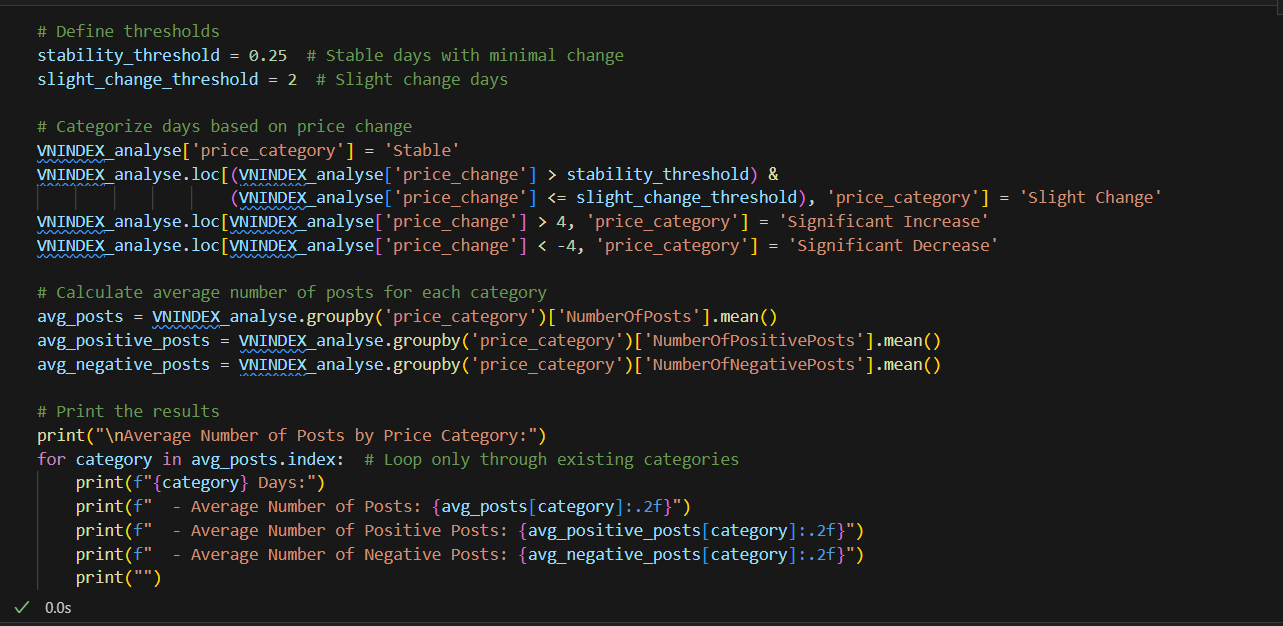
\includegraphics[width=1\linewidth]{images/C4_7.png}
\end{center}

\begin{figure}[H]
    \centering
    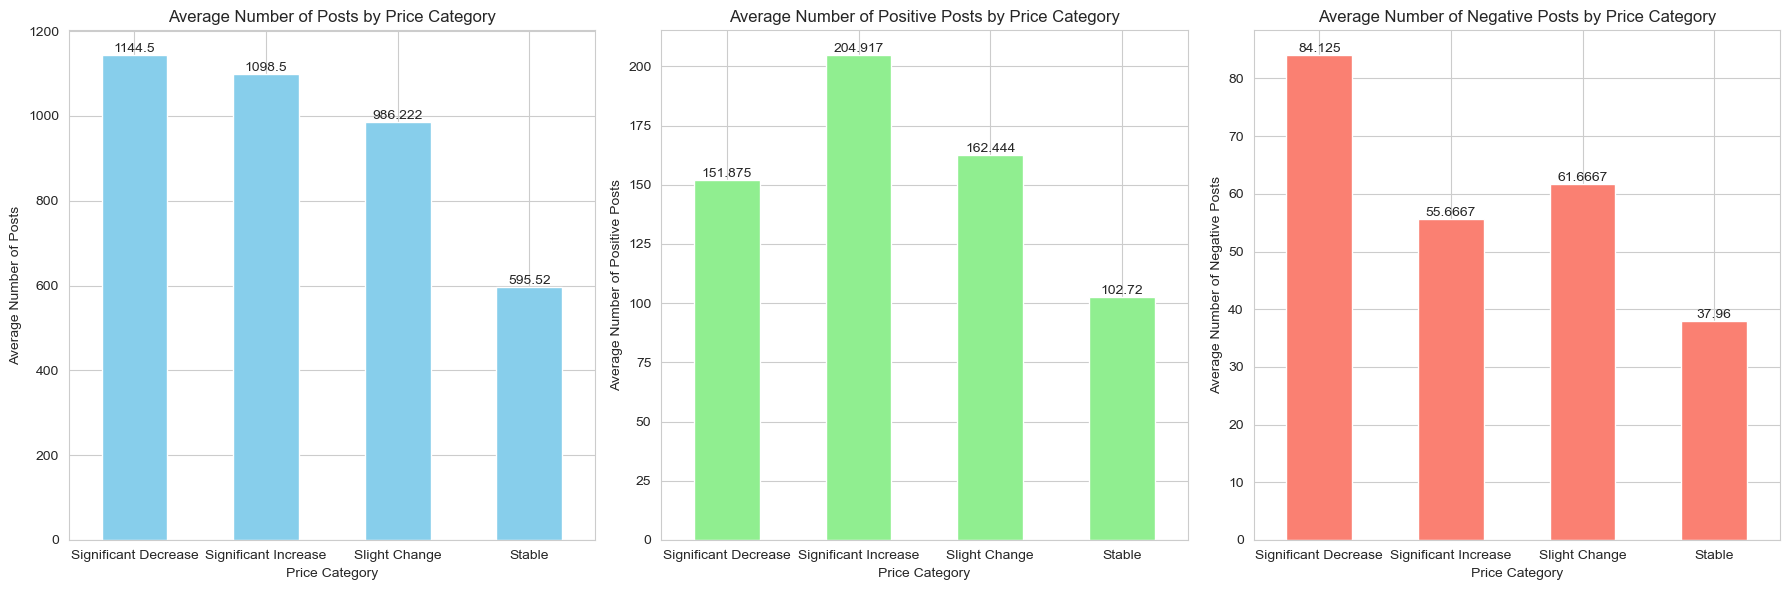
\includegraphics[width=1\linewidth]{images/C4_8.png}
    \caption{Biểu đồ số lượng bài viết theo sự thay đổi về giá}
    \label{fig:4.2}
\end{figure}

Kết quả cho thấy, vào những ngày VNINDEX giảm mạnh (\textit{Significant Decrease Days}), số lượng bài viết trung bình đạt mức cao nhất (1144.50). Điều này phản ánh sự quan tâm đặc biệt từ cộng đồng đầu tư khi thị trường có biến động giảm đáng kể. Đáng chú ý, số lượng bài viết tích cực (151.88) và tiêu cực (84.12) đều tăng cao, cho thấy các ý kiến thảo luận về biến động giảm không chỉ tập trung vào mặt tiêu cực mà còn bao hàm cả những cảm xúc lạc quan.\\

Ngược lại, vào những ngày VNINDEX tăng mạnh (\textit{Significant Increase Days}), số lượng bài viết tích cực đạt mức cao nhất (204.92), phản ánh sự lạc quan và kỳ vọng lớn từ cộng đồng đầu tư trong bối cảnh thị trường khởi sắc. Đồng thời, số lượng bài viết tiêu cực lại rất thấp (55.67), cho thấy tâm lý chung khá tích cực trong các phiên tăng mạnh.\\

Trong khi đó, vào những ngày thị trường ổn định (\textit{Stable Days}), số lượng bài viết trung bình chỉ đạt 595.52, thấp nhất trong tất cả các loại ngày. Điều này cho thấy khi thị trường không có biến động lớn, mức độ quan tâm từ cộng đồng giảm đáng kể. Số lượng bài viết tích cực (102.72) và tiêu cực (37.96) cũng duy trì ở mức thấp, thể hiện sự trầm lắng trong thảo luận khi không có sự kiện nổi bật xảy ra.

\subsubsection{Hệ số tương quan giữa VNINDEX và số bài đăng}
Đầu tiên ta cần biết giá trị trung bình và độ lệch chuẩn của VNINDEX trong dữ liệu:

\begin{center}
    \centering
    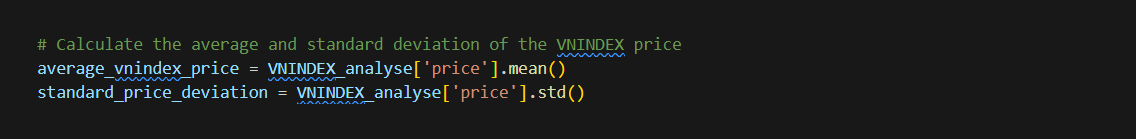
\includegraphics[width=0.85\linewidth]{images/C2_pic31.png}
\end{center}
\begin{center}
    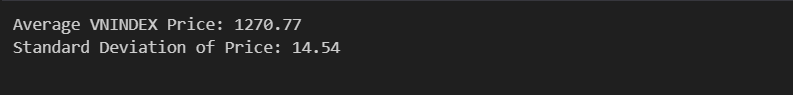
\includegraphics[width=0.75\linewidth]{images/C2_pic32.png}
\end{center}

Kết quả cho thấy giá trị trung bình của VNINDEX trong khoảng thời gian 2 tháng là 1270.77, với độ lệch chuẩn 14.54. Điều này cho thấy VNINDEX có sự biến động không quá lớn trong giai đoạn này, mức giá trung bình tương đối ổn định và độ lệch chuẩn cho thấy sự dao động giá vừa phải. Ta thực hiện tính toán hệ số tương quan giữa phàn trăm thay đổi của số lượng bài đăng và giá trị cổ phiếu, sử dung hàm \texttt{pct\_change()} và \texttt{corr()} có sẵn trong \texttt{pandas}.

\begin{center}
    \centering
    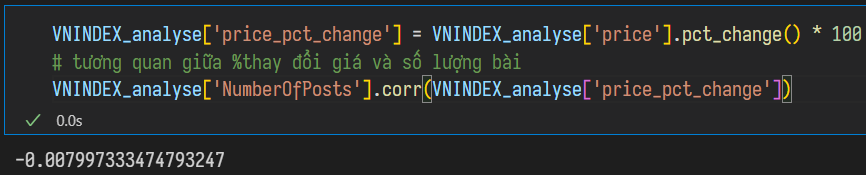
\includegraphics[width=0.75\linewidth]{images/C4_1.png}
\end{center}

Kết quả cho thấy hệ số tương quan giữa sự thay đổi phần trăm giá trị và số lượng bài đăng là -0.008, cho thấy chẳng có mối quan hệ giữa hai yếu tố này.\\

Kết quả cho thấy tính toán của ta có thể đã có vẫn đề, bởi theo như quan sát từ trước sự thay đổi trong giá trị cổ phiếu thường dẫn theo số lượng bài đăng sẽ tăng cao. Ta nhận thấy, số lượng bài viết đều có xu hướng tăng khi giá tăng hoặc giá giảm. Việc chỉ dùng giá trị thay đổi thuần để tính hệ số tương quan như các lần thực hiện trước đó là chưa chính xác, vì nó bỏ qua yếu tố rằng cả biến động tăng và giảm đều có thể kích thích sự thảo luận từ phía cộng đồng nhà đầu tư. Vậy nên ta phải tính theo \textbf{giá trị tuyệt đối phần trăm thay đổi giá trong ngày}, tức phải bổ sung giá trị tuyệt đối.

\begin{center}
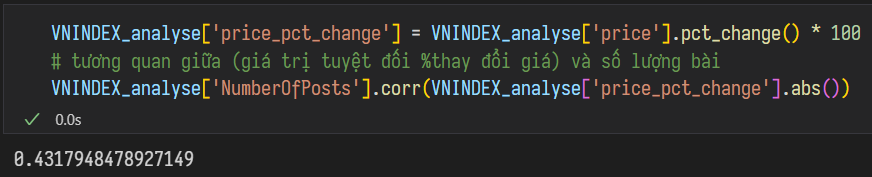
\includegraphics[width=0.75\linewidth]{images/C4_3.png}
\end{center}

Đúng như những nhận định và dự đoán trước đó, số lượng bài viết giờ đã mối liên kết rõ ràng hơn với chỉ số VNINDEX nói riêng và các mã cổ phiếu khác nói chung. Xu hướng này cho thấy sự quan tâm của nhà đầu tư đối với thị trường chứng khoán được thể hiện rõ ràng thông qua hoạt động thảo luận trên các diễn đàn. Tuy nhiên, giá trị chỉ 0.432 cũng chỉ ra rằng mối liên kết này chưa phải mối liên kết mạnh mẽ.\\

Để thể hiện rõ hơn xu hướng, ta có thể vẽ biểu đồ Scatter plot:
\begin{figure}[H]
    \centering
    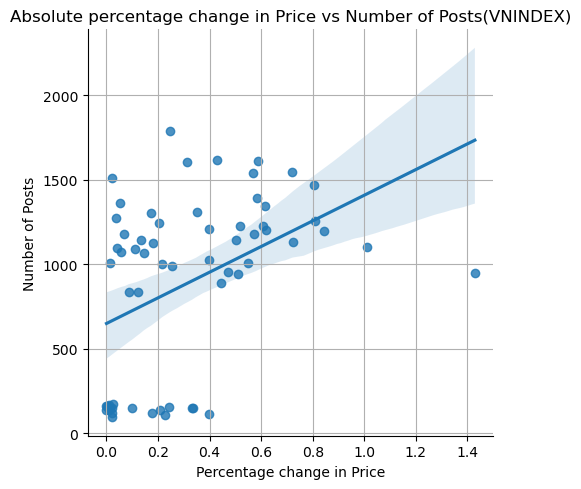
\includegraphics[width=0.55\linewidth]{images/C4_5.png}
    \vspace{-1em}
    \caption{Scatter plot thể hiện Tương quan giữa Phần trăm thay đổi giá và Số lượng bài viết}
    \label{fig:4.4}
\end{figure}

Thực hiện tương tự với số lượng bài đăng tích cực và tiêu cực với giá trị cổ phiếu:

\begin{figure}[H]
    \centering
    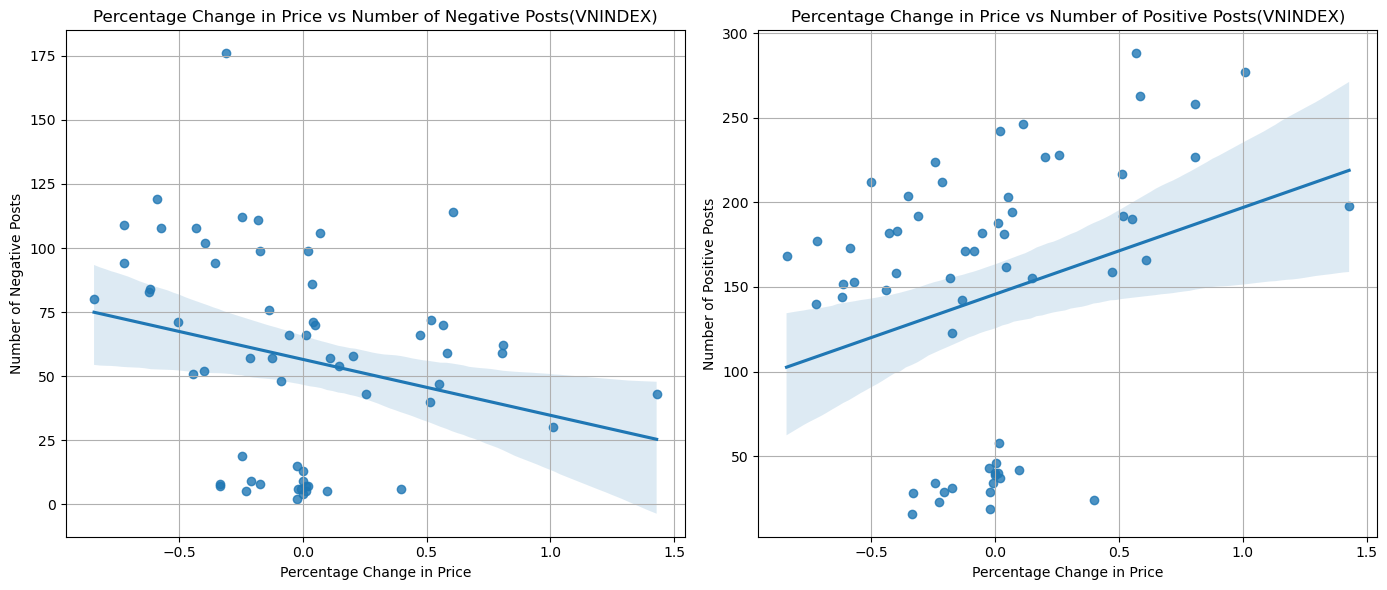
\includegraphics[width=1\linewidth]{images/C4_6.png}
    \caption{Tương quan giữa Phần trăm thay đổi giá và Số lượng bài viết Tích cực/Tiêu cực}
    \label{fig:4.5}
\end{figure}

Để ý rằng, trong ba biểu đồ trên luôn có một cụm chấm đứng rời rạc hẳn so với phần còn lại. Những vùng chấm đó là khi giá VNINDEX không đổi và số lượng bài đăng thấp. Ta dễ dàng thấy điều này hay xảy ra vào lúc cuối tuần. Như vậy, nếu ta chỉ xét khoảng thời gian giao dịch (tức từ 9h-15h hàng ngày, từ Thứ 2 đến Thứ 6), sự đồng pha thể hiện còn rõ ràng hơn với giá trị tương quan 0.67:

\begin{figure}[H]
    \centering
    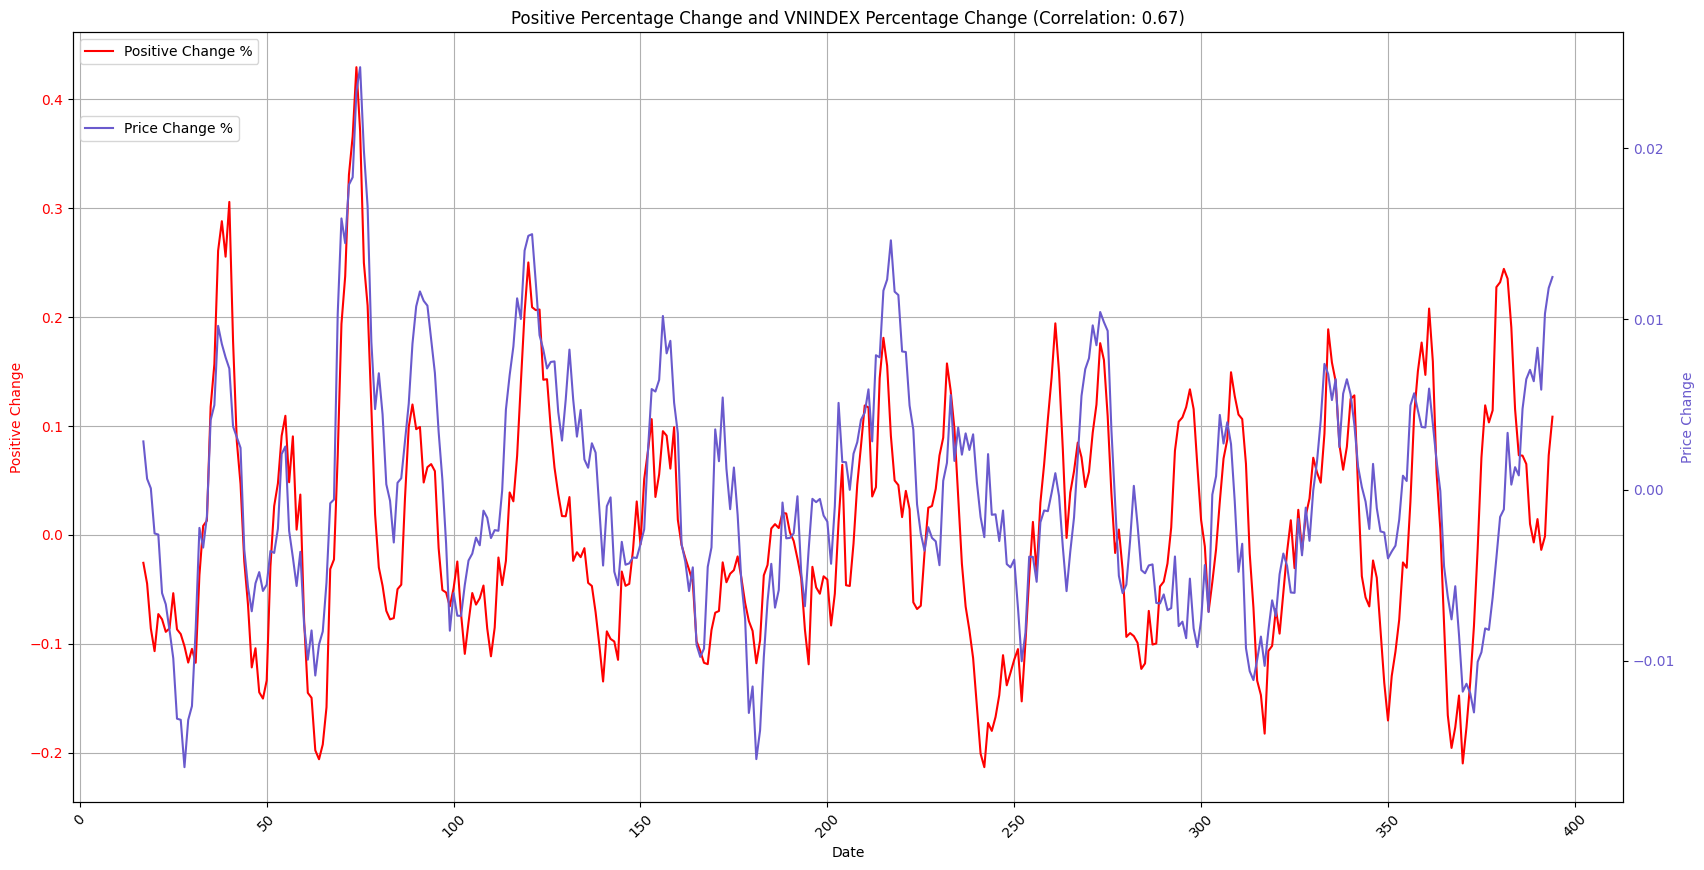
\includegraphics[width=1\linewidth]{images/plot-4.6-in.png}
    \caption{Diễn biến Phần trăm thay đổi giá và Số lượng bài viết Tích cực (Trong phiên)}
    \label{fig:4.6}
\end{figure}

Tóm lại, kết quả từ các biểu đồ cho thấy một xu hướng khá rõ ràng. Đường hồi quy của số lượng bài viết tiêu cực có độ dốc đi xuống, phản ánh mối quan hệ nghịch giữa số lượng bài viết tiêu cực và giá trị VNINDEX. Điều này cho thấy \textbf{khi VNINDEX tăng, số lượng bài viết tiêu cực có xu hướng giảm}.\\

Ngược lại, đường hồi quy của số lượng bài viết tích cực có độ dốc đi lên, chỉ ra mối quan hệ thuận với giá trị VNINDEX. \textbf{Khi VNINDEX tăng, số lượng bài viết tích cực cũng tăng theo}, phản ánh tâm lý lạc quan của nhà đầu tư trong những phiên thị trường khởi sắc.\\

Những xu hướng này \textbf{hoàn toàn phù hợp} với các dự đoán trước đó và được thể hiện một cách trực quan, rõ ràng qua biểu đồ, dù độ tương quan chưa phải rõ rệt.
